% https://www.scss.tcd.ie/~munnellg/projects/edge_detection.html
% https://northstar-www.dartmouth.edu/doc/idl/html_6.2/Sharpening_an_Image.html
% https://homepages.inf.ed.ac.uk/rbf/HIPR2/log.htm

Edge detection, vizinhança 4 8, laplaciano

Realce não direcional % http://www.dpi.inpe.br/spring/teoria/filtrage/filtragem.htm

\begin{figure}[H]
    \centering
    \begin{subfigure}{0.4\textwidth}
        \centering
        \begin{kmatrix}
    \matrix[square matrix]{
        0 & 0 & -1 & 0 & 0 \\
        0 & -1 & -2 & -1 & 0 \\
        -1 & -2 & 16 & -2 & -1 \\
        0 & -1 & -2 & -1 & 0 \\
        0 & 0 & -1 & 0 & 0 \\
    };
\end{kmatrix}
        \caption{~$h_1$}
        \label{fig:h1}
    \end{subfigure}%
    \begin{subfigure}{0.4\textwidth}
        \centering
        \begin{kmatrix}
    \matrix[square matrix]{
        -1 & -1 & -1 \\
        -1 & 8 & -1 \\
        -1 & -1 & -1 \\
    };
\end{kmatrix}
        \caption{~$h_5$}
        \label{fig:h5}
    \end{subfigure}

    \caption{??}
\end{figure}

\begin{figure}[H]
    \centering
    \begin{subfigure}{0.48\textwidth}
        \centering
        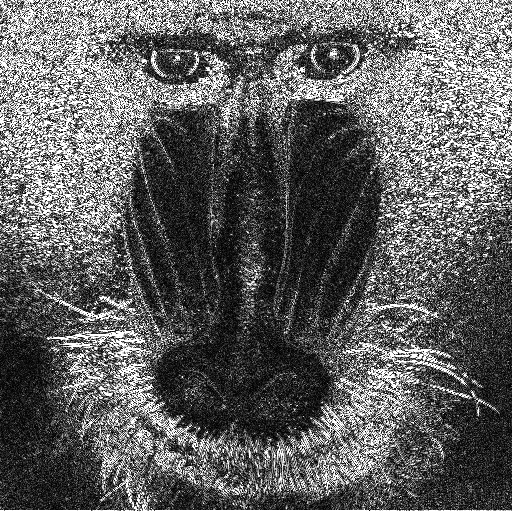
\includegraphics[width=0.9\textwidth]{imagens/baboon.png}
        \caption{Original: \texttt{baboon.png}.}
    \end{subfigure}\\[8pt]
    \begin{subfigure}{0.48\textwidth}
        \centering
        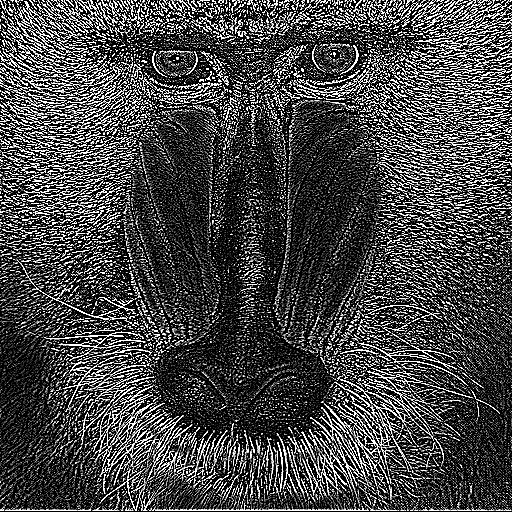
\includegraphics[width=0.9\textwidth]{resultados/baboon_h1.png}
        \caption{Convolução com ??.}
    \end{subfigure}%
    \begin{subfigure}{0.48\textwidth}
        \centering
        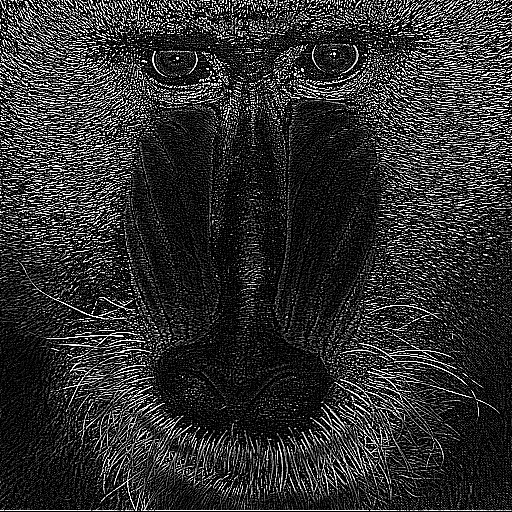
\includegraphics[width=0.9\textwidth]{resultados/baboon_h5.png}
        \caption{Convolução com ??.}
    \end{subfigure}

    \caption{??}
\end{figure}
